%&pdflatex
\documentclass[11pt, a4paper]{article}
\usepackage{graphicx}
\usepackage{amsmath}
\usepackage{listings}
\usepackage{minted}
\usepackage{color}   %May be necessary if you want to color links
\usepackage{hyperref}
\hypersetup{
    colorlinks=true, %set true if you want colored links
    linktoc=all,     %set to all if you want both sections and subsections linked
    linkcolor=magenta,  %choose some color if you want links to stand out
}

\title{\textbf{EE2703: Applied Programming Lab - Assignment No. 3}}

\author{
	\textbf{Name} : Abishek S \\
	\textbf{Roll Number} : EE18B001
}\date{\today}

\begin{document}

\maketitle
\section{Abstract}
The aim of this assignment is :
\begin{itemize}
\item To plot graphs and analyse data
\item To generate noise and study how it affects the given data
\item To use least squares fitting to model the data
\item To study the variation of mean squared error and noise
\end{itemize}
\usemintedstyle{manni}

\section{Assignment}
\subsection{Parts 1 and 2}
Importing relevant libraries
\begin{minted}[mathescape,escapeinside = ||,obeytabs,tabsize = 2]{python3}
import pylab as pl
import scipy.special as sp
import sys
\end{minted}
\hypertarget{g}{
Defining function g(t;A,B),  loading data from 'fitting.dat' and obtaining the true value of the function.}
\begin{minted}{python3}
def g(t,A = 1.05,B = -0.105):
	return A*(sp.jn(2,t)) + B*t

data = pl.loadtxt('./fitting.dat')
t = data[:,0]
Y = data[:,1:]
true_y  = g(t)
\end{minted}

\subsection{Part 3}
The function with different noise amounts is plotted along with it's true value.
\begin{minted}{python3}
sigma = pl.logspace(-1,-3,9)  #The Standard Deviations of noise
fig = pl.figure(0)
pl.title('Plot of Data')
pl.plot(t,pl.c_[Y,true_y])
pl.xlabel(r'$t$')
pl.legend(list(sigma) + ['true value'])
pl.grid(True)
pl.show()
\end{minted}

\begin{figure}[!htb]
   	\centering
   	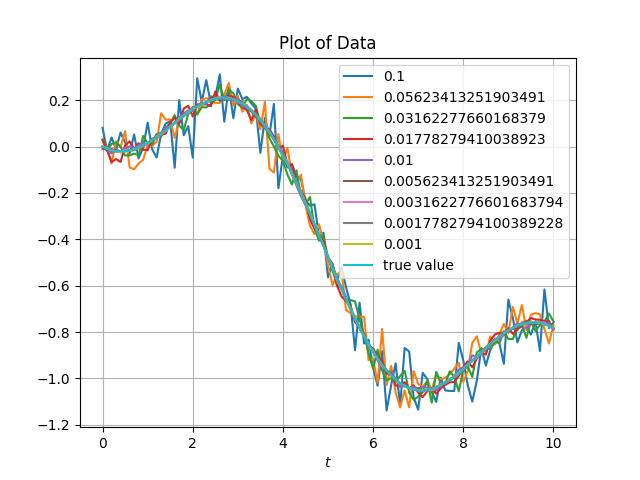
\includegraphics[scale=0.5]{dataplot.png}
   	\caption{Value vs Time, for different error amounts}
   	\label{fig:dataplot}
\end{figure} 

\subsection{Part 4}
We plot the true value of the function obtained from g(t;A,B) we already defined \hyperlink{g}{in Part 2}.
\begin{minted}{python3}
fig = pl.figure(0)
pl.title('Plot of True value')
pl.plot(t,true_y,label = 'true value') 
pl.xlabel(r'$t$')
pl.ylabel(r'$1.05*J(t)-0.105t$')
pl.grid(True)
pl.legend()
pl.show()
\end{minted}
\begin{figure}[!htb]
   	\centering
   	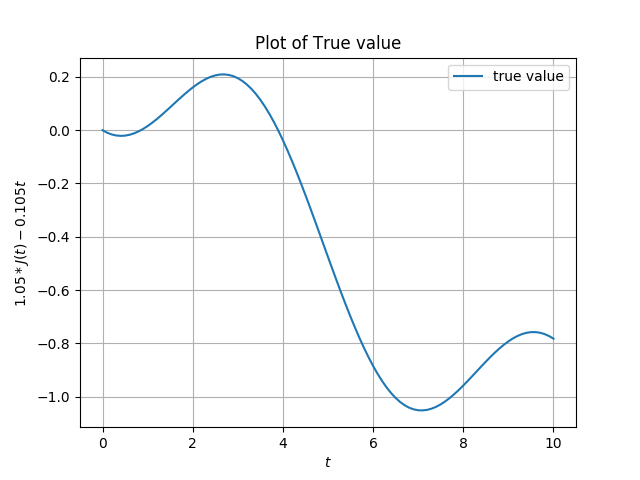
\includegraphics[scale=0.5]{truevalue.png}
   	\caption{True value of Function obtained without Matrix multiplication}
   	\label{fig:truevalue}
\end{figure}
   
\subsection{Part 5}
We plot errorbars along with the data in column 1.
\begin{minted}{python3}
fig = pl.figure(1)
pl.title('Errorbars')
pl.plot(t,pl.c_[true_y,Y[:,0]])
stdev = pl.std(Y[:,0]-true_y)
pl.errorbar(t[::5],Y[::5,0],stdev,fmt='ro')
pl.xlabel(r'$t$')
pl.legend(['True value','Noisy curve'])
pl.show()
\end{minted}

\begin{figure}[!htb]
   	\centering
   	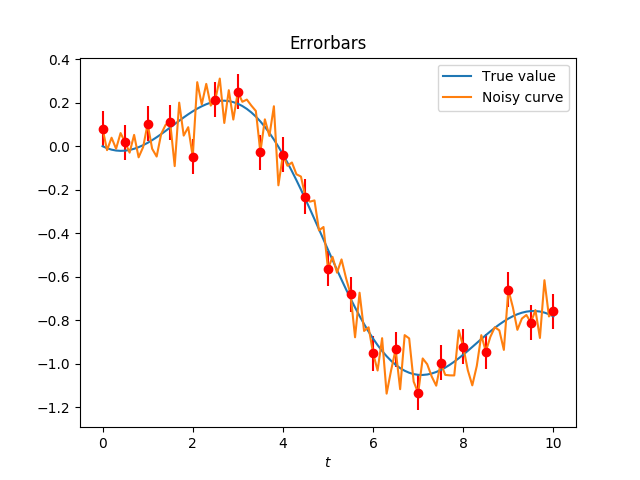
\includegraphics[scale=0.5]{errorbar.png}
   	\caption{Function with Error Bars}
   	\label{fig:errorbars}
\end{figure}

\subsection{Part 6}
We define new g function which calculates values through matrix multiplication.
\begin{equation}\label{eq:1}
g\_new(t,A,B) = 
\begin{pmatrix}
J_2(t1)  & t_1 \\
... & ... \\
J_2(t_m) & t_m \\
\end{pmatrix}
\begin{pmatrix}
A \\ B\\
\end{pmatrix}
\end{equation}
\begin{minted}{python3}
def g_new(t,A = 1.05,B = -0.105):
	mat = pl.c_[sp.jn(2,t),t]
	param = pl.array([A,B])
	return pl.matmul(mat,param)

true_y_new = g_new(t)
if (true_y == true_y_new).all() == True:
	print('The two functions are equal')
else:
	print('The functions are not equal')
\end{minted}

\begin{figure}[!htb]
   	\centering
   	
\includegraphics[scale=0.5]{isEqual.png}
   	\caption{Output of comparing the two vectors}
   	\label{fig:eisEqual}
\end{figure}

\subsection{Part 7}
We find mean squared error between data in first column and the assumed model.
\begin{minted}[mathescape]{python3}
A_list = pl.linspace(0,2,21)
B_list = pl.linspace(-0.2,0,21)

#E[i,j] stores mean squared error for parameters A = A_list[i],B = B_list[j]
E = [[(1/len(true_y)) * sum(map(lambda x: x**2,Y[:,0]-g_new(t,a,b))) 
					for b in B_list] for a in A_list]
\end{minted}

\subsection{Part 8}
We plot the contour plot of $E_{ij}$ and we find that intensity of curves indicate the presence of one critical point (minima). We also mark the value of A = 1.05, B = -0.105 in the plot.
\begin{minted}[mathescape]{python3}
fig = pl.figure(2)
pl.title('Contour Plot')
pl.contour(A_list,B_list,E,40)
pl.plot(1.05,-0.105,'ro',label = 'Exact Value')
pl.annotate(s = 'Exact Value',xy = [0.8,-0.1])
pl.show()
\end{minted}

\begin{figure}[!htb]
   	\centering
   	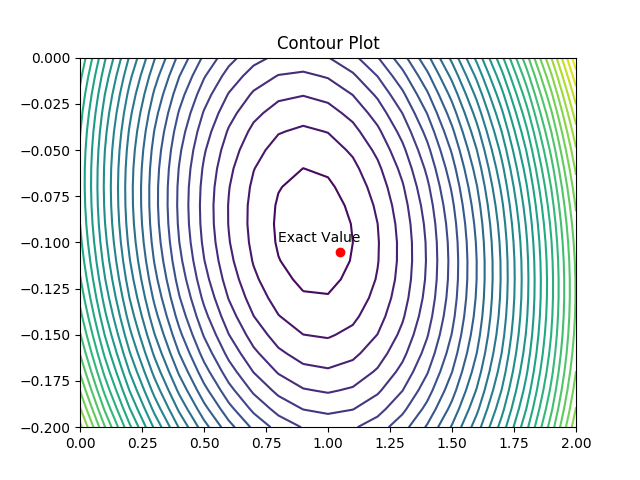
\includegraphics[scale=0.5]{contour.png}
   	\caption{Contour plot of $E_{ij}$}
   	\label{fig:contour}
\end{figure}

\subsection{Parts 9 and 10}
We estimate A and B values from linear least squares fitting for data in all columns (with different noise amounts).\\
We find the A and B estimated for data of column 1.
\begin{minted}{python3}
(A,B),(mse),*_ = pl.linalg.lstsq(pl.c_[sp.jn(2,t),t],Y[:,0],rcond = None)
print('A : ',A)
print('B : ',B)
\end{minted}

\begin{figure}[!htb]
   	\centering
   	
\includegraphics[scale=0.5]{A_and_B.png}
   	\caption{Output for predicted A and B}
   	\label{fig:A_and_B}
\end{figure}

We then generate a  mean squared error vs noise sigma plot. We also mark the absolute difference between original A,B and the predicted A,B for different columns of data.
\begin{minted}[mathescape]{python3}
mse_list = []
pred_A = []
pred_B = []
for i in range(Y.shape[1]):
	(a,b),(mse),*_ = pl.linalg.lstsq(pl.c_[sp.jn(2,t),t],Y[:,i],rcond = None)
	mse_list.append(mse)
	pred_A.append(a)
	pred_B.append(b)

pred_A = pl.array(pred_A)
pred_B = pl.array(pred_B)

fig = pl.figure(3)
pl.title('Error vs Noise')
pl.plot(sigma,mse_list,label = 'Mean Squared Error')
pl.plot(sigma,pl.absolute(pred_A-1.05),'ro',label = '|Ao-Ap|')
pl.plot(sigma,pl.absolute(pred_B+0.105),'go',label = '|Bo-Bp|')
pl.legend()
pl.xlabel(r'Noise sigma')
pl.show()
\end{minted}

\begin{figure}[!htb]
   	\centering
   	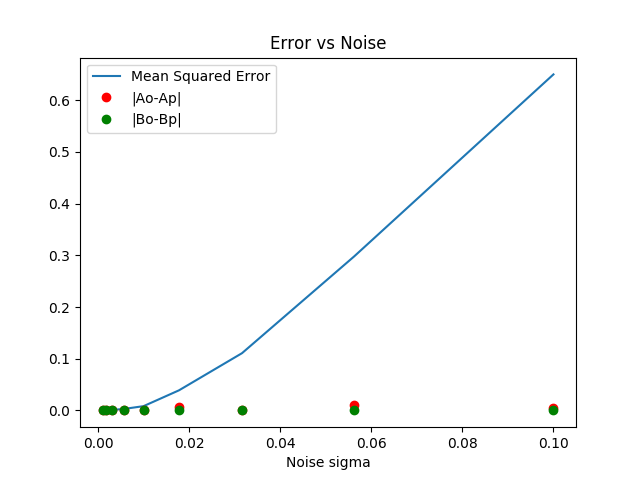
\includegraphics[scale=0.5]{errorvsnoise.png}
   	\caption{Error VS Noise}
   	\label{fig:errorvsnoise}
\end{figure}

\subsection{Part 11}
We now plot the above graph of error vs noise in log-log scales. \\
The blue line indicates that the mean squared error varies almost linearly with noise sigma in log-log scale.
\begin{minted}[mathescape]{python3}
fig = pl.figure(4)
pl.title('Log Error vs Log Noise')
pl.loglog(sigma,mse_list,label = 'Log of Mean Squared Error')
pl.loglog(sigma,pl.absolute(pred_A-1.05),'ro',label = 'log|Ao-Ap|')
pl.loglog(sigma,pl.absolute(pred_B+0.105),'go',label = 'log|Bo-Bp|')
pl.legend()
pl.xlabel(r'Noise sigma')
pl.show()
\end{minted}

\begin{figure}[!htb]
   	\centering
   	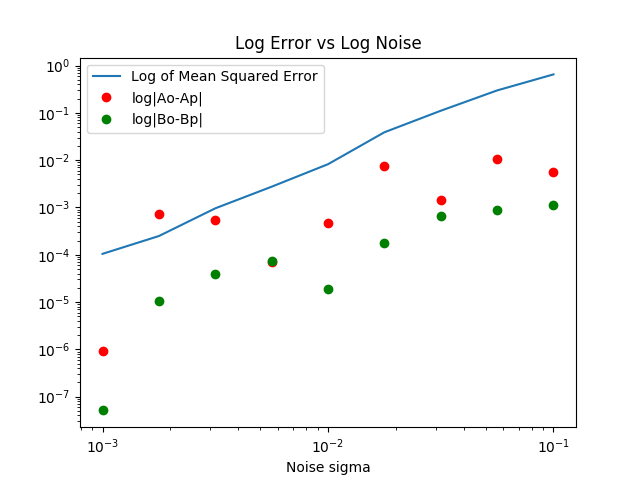
\includegraphics[scale=0.5]{loglogplot.png}
   	\caption{Log Error VS Log Noise}
   	\label{fig:loglogplot}
\end{figure}

\section{Conclusions}
\begin{itemize}
	\item Plotting graphs can make it easier to analyse a situation.
    \item Least Squares Fitting can be used to estimate the parameters of the linear model for an overdetermined system of equations.
    \item $\log(error)$ varies nearly linearly with $\log(noise)$.
\end{itemize}

\end{document}
